%\section{Experiment}\label{sec:experiment}

\section{Empirical results} \label{sec:experiment}

To measure the efficiency of our approach, we conducted two empirical studies. The first takes into consideration the whole system 
(PEPs and PDPs) and evaluates the performance improvement regarding decision making process. The request processing time, 
for each splitting criterion is compared to the processing time of the initial architecture implementing the global policy (the evaluation 
that considers the global policy, is denoted (IA), the ``Initial Architecture''). The second empirical study focuses only on the PDPs in isolation to measure the gain in performance independently from system's requests. To make 
such study of PDPs in isolation, we use XEngine \cite{Xengine}. The objective of the second study is to see how our approach can be combined with XEngine and 
how this impacts the performance.
\\
The first subsection introduces our empirical studies and presents the tool that supports our approach. The remaining two sections present and discuss the results of the two empirical studies.  

\subsection{Empirical Studies and PolicySplitter Tool}
The empirical studies were conducted using the following systems (They are presented in details in \cite{testcase}):
\begin{itemize}	
\item LMS: The library management system offers services to manage books in a public library.
\item VMS: The virtual meeting system offers simplified web conference services. The virtual meeting server allows the organization of work meetings on 
a distributed platform.
\item ASMS (Auction Sale Management System): allows users to buy or sell items online. A seller can start an auction by submitting a description of the
item he wants to sell and a minimum price (with a start date and an ending date for the auction). Then usual bidding process can apply and people can bid 
on this auction. One of the specificities of this system is that a buyer must have enough money in his account before bidding.
\end{itemize}
We started by a processing step, in which we have augmented the rules number in the three original policies for these studies, as it would be difficult
 to observe a performance improvement results with systems including few rules. In our evaluations, LMS policy contains 720 rules, VMS has 945 rules while ASMS implements 1760 rules. 
The rules that we have added do not modify the system behavior as they are conform to the specifications. Our evaluations were carried out on a desktop PC, running Ubuntu 10.04 with Core i5, 2530 Mhz processor, and 4 GB of RAM. 
\\
We have implemented the PolicySplitter tool in Java. PolicySplitter enables splitting policies according to the chosen splitting criteria. 
It is available for download from \cite{splitter}.
The execution time of the tool is not considered as a performance factor as it takes up to few seconds (for very large policies) to perform the splitting 
according to all SCs. Moreover the refactoring process is executed only once to create a configuration that supports a selected splitting criterion and more importantly
the splitting is not performed on runtime.


\subsection{Performance Improvement Results}
For the 3 evaluation studies, we generated all sets of policies for all the splitting criteria that we have defined in Section III.
The decision Engine in our three case studies is based on Sun XACML PDP implementation \cite{sunxacml}. We choose to use Sun XACML PDP instead of XEngine in order to prove the effectiveness
 of our approach when compared to the traditional architecture.



% To run the experiments, we used a configuartion file that maintains the list of policies used for requests evaluation. 
% For the initial architecture, the configuration file contains one policy. Sun XACML PDP uses this configuration file to select to XACML files that constitute the policy.

For each system, we executed all functional and security tests. This process is repeated ten times in order to reduce randomness.
These tests enable validating all the system functions and checking all policy rules (more information 
about the way these tests were created can be found in our previous paper \cite{testcase}).  
For each splitting criteria, we have conducted functional tests to generate 
requests that trigger all the PEPs in the three evaluation studies. The test generation step is presented in \cite{testcase} as well.
We applied this process to each splitting criterion and calculated the average execution time. We only consider the execution time of the PDP and we do not include the executions of the system functions. 
\\
The results are shown in Figure \ref{fig:processing time}. They show the execution time for each splitting criterion and for the initial architecture (IA).
Note that the results are ranked from the largest processing duration to the smallest one. From the Figure \ref{fig:processing time}, we can make two main observations:

\begin{itemize} 
\item Compared to the initial architecture (IA), the evaluation time is considerably reduced for all splitting criteria. This is consistent with our 
initial intuition. In fact, splitting the policy into small policies improves the processing duration.
\item The splitting criteria \normalsize $SC=< Action, Resource>$ enables to have the best evaluation duration. 
In fact, the PEPs in the 3 empirical studies are scattered in the applications by a categorization
 that is based on $<Action, Resource>$. This pleads in favor of adopting a
 splitting criteria that takes into account the PEP-PDP synergy property.
\end{itemize} 
\begin{figure*}
  \centering
{\label{fig:gull}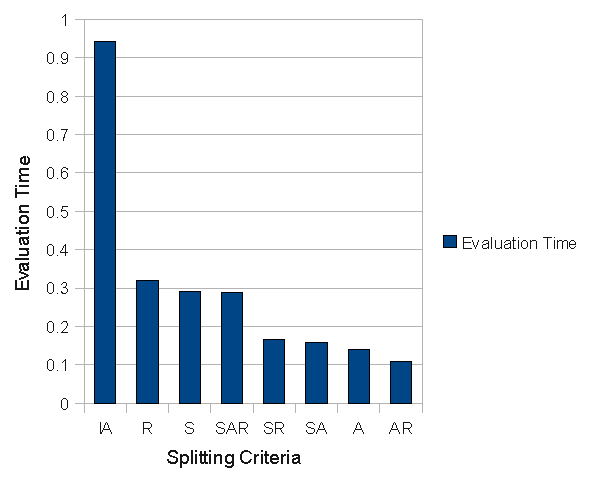
\includegraphics[width=0.33\textwidth]{LMS.pdf}}                
{\label{fig:VMS}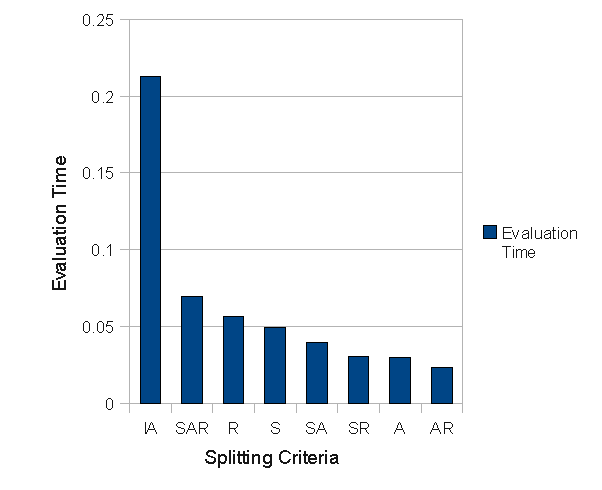
\includegraphics[width=0.33\textwidth]{VMS.pdf}}
{\label{fig:ASMS}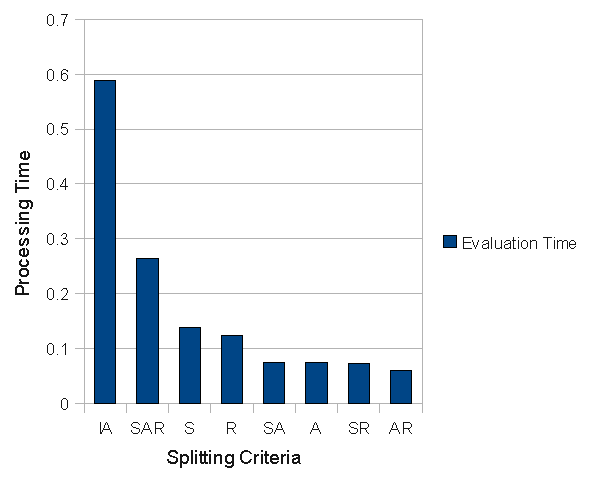
\includegraphics[width=0.33\textwidth]{ASMS.pdf}}
  \caption{Processing Time for our 3 systems LMS, VMS and ASMS}
  \label{fig:processing time}
\end{figure*}
\begin{figure}[!h]
  \centering
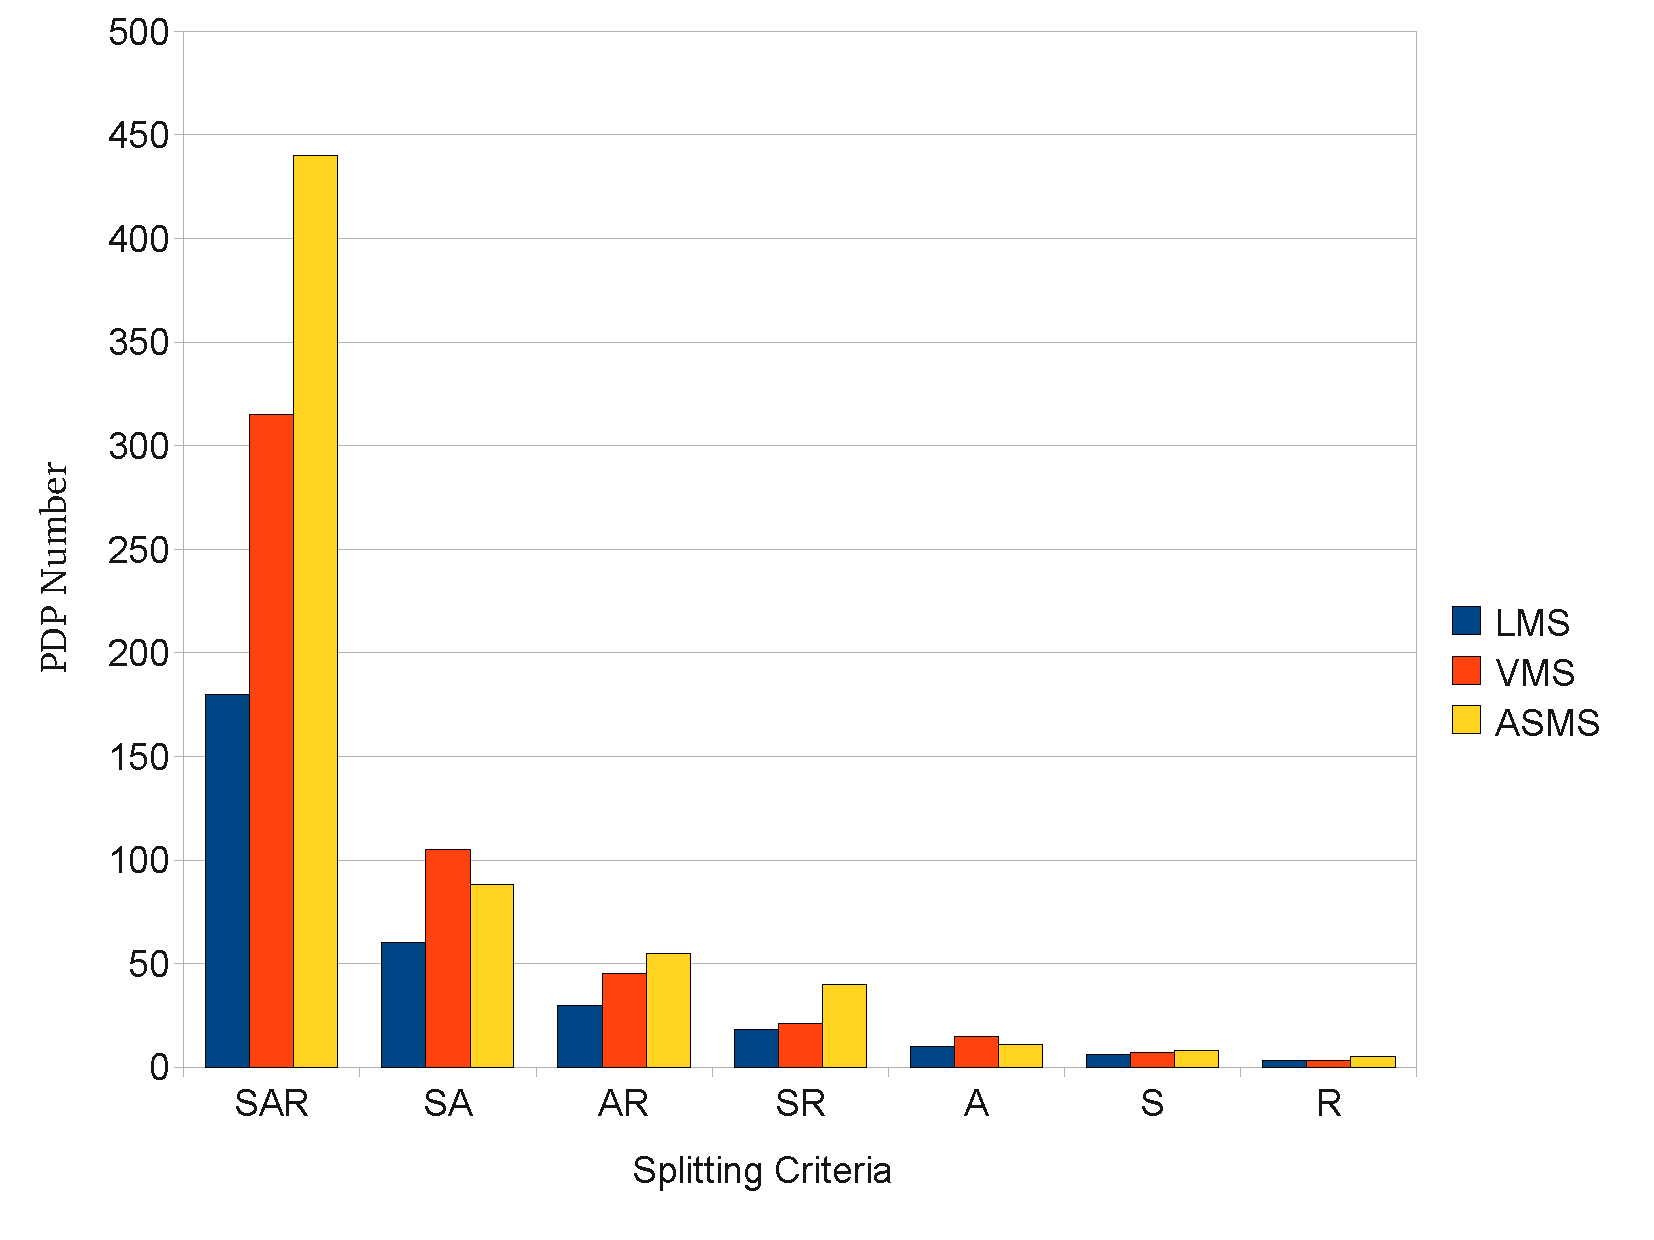
\includegraphics[width=8.5cm, height=6cm]{pdpnumber.pdf}
\begin{center}
\caption{PDP Number According to Splitting Criteria}
\label{pdpnumber}
\end{center}
\end{figure} 
A refactoring process that engenders a huge number of small policies may lead to integrity issues. For this sake, 
we propose to evaluate PDPs number generated by each splitting criterion, to study the impact of the refactoring process on the initial policy. 
For the 3 XACML studies, we executed PoliySplitter on the 3 initial policies and we generated the number of resulting policies, in each study. 
As highlighted by Figure \ref{pdpnumber}, we notice that there are three
 categories of results: The splitting criterion $SC_{1}$ that consists in a single target element, 
leads to a small number of PDPs, the splitting criterion $SC_{2}$ produces a reasonable number of PDPs whereas $SC_{3}$ leads to a huge 
number od PDPs. The splitting criterion $SC_{2}$, thus appears as a good tradeoff in terms of performance and number of 
PDPs generated: In our evaluation studies, $SC=<Action, Resource>$ is the best criterion, both in terms of performances and low number of PDPs.

\subsubsection{Performance improvement with XEngine}
The goal of this empirical study is to show the impact of combining XEngine with our approach. In fact, XEngine improves dramatically 
the performance of the PDP \cite{Xengine}, mainly for 3 reasons:

\begin{itemize}
\item It uses a refactoring process that transforms the hierarchical structure of the XACML policy to a flat structure. 
\item It converts multiple combining algorithms to single one.
\item It lies on a tree structure that minimizes the request processing time.
\end{itemize}
We propose to use XEngine conjointly with the refactoring process presented in this work:
We have evaluated our approach in 2 settings:
\begin{itemize}
\item Considering evaluations with a decision engine, based on SUN PDP, with split policies and with the initial policy.  
\item Considering evaluations with a decision engine, based on XEngine rather than Sun PDP, with split policies and with the initial policy as well.  
\end{itemize}
We have measured the processing time (in ms) of a randomly generated set of 10,000 requests. For request generation, we have used the technique presented 
in \cite{request}. The request time processing is evaluated for LMS, VMS, ASMS. The results are presented in Table II, III and IV.




From the different tables, we can observe that, when used with a decision engine based on XEngine rather than Sun PDP, our proposed approach provides more performance improvement. 
For the splitting criteria $SC=<Action>$, in the LMS system, the evaluation time is reduced about 9 times: from 2703 ms to 290 ms with XEngine. This empirical observation plead in favour of applying our proposed
 refactoring process with XEngine.

